\documentclass{article}
\usepackage[utf8]{inputenc}
\usepackage{amsmath}
\usepackage{geometry}
\geometry{
 a4paper,
 total={182mm,257mm},
 left=14mm,
 top=20mm,
 }
 \usepackage{siunitx}
 \usepackage{amsthm}
 \usepackage[utf8]{inputenc}
 \usepackage[italian]{babel}
\usepackage[T1]{fontenc}
\usepackage{amssymb}
\usepackage{physics}
\usepackage{commath}
\usepackage{tikz}
\usepackage{pgfplots}
\pgfplotsset{compat=1.15}
\usepackage{graphicx}
\graphicspath{ {Immagini/} }
\usepackage{float}
\usepackage{hyperref}
\hypersetup{
    colorlinks=true,
    linkcolor=red,
    citecolor=green
    filecolor=magenta,      
    urlcolor=cyan,
}


%Theorem Environments
\newtheorem{thm}{Teorema}[section]
\newtheorem{lem}[thm]{Lemma}
\newtheorem{property}{Proprietà}[section]
\newtheorem{defn}{Definizione}[section]
\newtheorem{prop}[defn]{Proposizione}
\newtheorem{example}{Esempi}[subsection]
\newtheorem{exerc}[example]{Esercizi Svolti}

%Commandi di Formattazione
\newcommand{\noi}{\noindent}
\newcommand{\note}{\noindent {\quad \bf \underline{Osservazione:}} \quad}
\newcommand{\eg}{\noindent {\bf \underline{Esempio:}} \quad}
\newcommand{\bfemph}[1]{\textbf{\textit{#1}}}
\renewcommand{\emph}[1]{\bfemph{#1}}

%Number Sets
\newcommand{\R}{\mathbb{R}}
\newcommand{\C}{\mathbb{C}}
\newcommand{\Z}{\mathbb{Z}}
\newcommand{\Q}{\mathbb{Q}}

%Shortcuts
\newcommand{\then}{\ensuremath{\Rightarrow}}
\newcommand{\twopartdef}[4]
{
	\left\{
		\begin{array}{ll}
			#1 & \mbox{se } #2 \\
			#3 & \mbox{se } #4
		\end{array}
	\right.
}

%Vectors
\renewcommand{\i}{\vu{i}}
\renewcommand{\j}{\vu{j}}
\renewcommand{\k}{\vu{k}}
\renewcommand{\a}{\va{a}}
\renewcommand{\b}{\va{b}}
\renewcommand{\c}{\va{c}}
\renewcommand{\v}{\va{v}}
\renewcommand{\u}{\va{u}}
\newcommand{\s}{\va{s}}
\renewcommand{\t}{\va{t}}
\newcommand{\verst}{\vu{t}}
\newcommand{\versr}{\vu{r}}
\renewcommand{\r}{\va{r}}
\newcommand{\tauvs}{\vu{\tau}}
\newcommand{\tauvt}{\va{\tau}}
\newcommand{\normvs}{\vu{n}}
\newcommand{\N}{\va{N}}
\newcommand{\g}{\va{g}}
\newcommand{\F}{\va{F}}
\newcommand{\f}{\va{f}}
\newcommand{\M}{\va{M}}
\renewcommand{\l}{\va{l}}
\newcommand{\p}{\va{p}}
\renewcommand{\P}{\va{P}}
\renewcommand{\L}{\va{L}}


\renewcommand{\c}{\overline{c}}
\title{Termodinamica}
\author{Roberto Gargiulo}
\date{Ultimo Aggiornamento: \today}


\begin{document}

\maketitle
\tableofcontents
\pagebreak

\section{Introduzione}
\subsection{Termologia}
Lo studio della termodinamica si basa sulla possibilità di raggiungere un'equilibrio, enunciata dal \textbf{principio zero}.\\
Un \textbf{sistema termodinamico} è costituito da una porzione di spazio materiale, separata in qualche modo dall'ambiente circostante. L'insieme di ambiente e sistema è noto come \textbf{universo termodinamico}.
Gli equilibri termodinamici compongono uno \textbf{spazio termodinamico} descritto da un certo numero di variabili (dette \textbf{grandezze termodinamiche}), tra le quali:
\begin{enumerate}
    \item Pressione
    \item Temperatura
    \item Volume
    \item Energia Interna
    \item Entropia
\end{enumerate}
\begin{defn}[Equilibrio Termodinamico]
L'equilibrio di un sistema termodinamico è costituito da tre equilibri che il sistema deve raggiungere:
\begin{enumerate}
    \item \textbf{Equilibrio Meccanico}, a cui corrisponde l'assenza di movimento macroscopico ed è caratterizzato dalla pressione, si raggiunge quando la pressione esterna è uguale a quella interna.
    \item \textbf{Equilibrio Chimico}, a cui corrisponde l'assenza di reazioni chimiche e trasformazioni di fase, a cui corrisponde il potenziale chimico, si raggiunge quando il potenziale chimico dei reagienti $\mu_A$ è uguale a quello dei prodotti $\mu_B$.
    \item \textbf{Equilibrio Termico}, quando la temperatura dell'ambiente e quella del sistema sono le stesse.
\end{enumerate}
\end{defn}

Queste tre grandezze sono \textbf{intensive} in quanto non dipendono dalle dimensioni del sistema o dalla quantità di materia. Le grandezze che dipendono dalle dimensioni e dalla quantità di materia sono dette \textbf{estensive} (additive) e includono massa, volume, entropia ed energia interna. Le prime sono grandezze valide per l'intero sistema, mentre le seconde variano a seconda della parte del sistema che consideriamo (il volume delle parti di un sistema corrisponde alla somma dei volumi, mentre la pressione di un sistema non è la somma delle pressioni di sue parti).\\
\note Per \textbf{pressione esterna} intendiamo la quantità:
\[p^{(e)}=\frac{\abs{\F^{(e)}\cdot\va{n}}}{A}\]
Con $\F^{(e)}$ forza esterna ed $\va{n}$ vettore normale rispetto alla superficie A. Solo negli stati di equilibrio meccanico (generalmente anche termodinamico) vale $p^{(e)}=p$.

\paragraph{Equazione di Stato}
L'\textbf{equazione di stato} di un sistema termodinamico è un'equazione del tipo:
\[t=t(p,V)\quad p=p(t,V)\]
Ossia una relazione tra pressione, volume e temperatura.
\begin{defn}[Varianza]
La varianza di un sistema termodinamico corrisponde al numero di gradi di libertà di quel sistema, ossia il numero di grandezze termodinamiche necessario a descriverlo. 
\end{defn}
Utilizzando la \textbf{Regola di Gibbs} possiamo calcolare la varianza di un sistema come segue:
\begin{equation}
    \boxed{v=n-f+2}
\end{equation}
Dove n è il numero di componenti (sostanze) ed f il numero di fasi. Quando $v=0$ il sistema si trova nel suo \textbf{punto triplo}, ossia un punto particolare dello spazio termodinamico determinato da specifiche coordinate di volume, pressione e temperatura. \\

Analizziamo ora più in dettaglio il significato di temperatura, una sua definizione operativa e il principio zero.
\begin{defn}[Principio Zero (dell'Equilibrio Termodinamico)]
Se due sistemi A e B sono in equilibrio termico con un sistema C, allora A e B sono in equilibrio termico tra di loro.
\end{defn}
\paragraph{Definizione Operativa di Temperatura}
\begin{enumerate}
    \item Nota una grandezza X (detta \textbf{caratteristica termometrica}) che caratterizza un certo fenomeno ed è variabile rispetto alla temperatura solamente, possiamo definire $t(X)$ come \textbf{funzione termometrica}.
    \item Deve esistere un punto fisso a cui si può attribuire con alta precisione un certo valore arbitrario, il punto fisso campione è il \textbf{punto triplo dell'acqua}, un punto dello spazio termodinamico ben definito. 
\end{enumerate}
In particolare, la scala Celsius si può definire nel seguente modo, per quanto limitato:
\begin{enumerate}
    \item Costruiamo un termometro formato da un recipiente d'acqua (\textit{bulbo}) collegato a un tubo lungo e sottile (capillare) contenente mercurio.
    \begin{figure}[H]
        \centering
        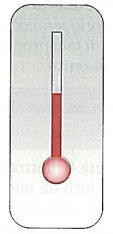
\includegraphics[width=0.09\textwidth]{DefTemp1.png}
        \caption{Termometro a Mercurio}
    \end{figure}
    \item Si stabilisce quindi tra temperatura $t$ e lunghezza del capillare occupato (in quanto si considera tanto sottile che il mercurio si possa espandere solo lungo la direzione del capillare e non le altre) una relazione lineare del tipo $t=aL+b$. Per determinare i valori di a e b è quindi necessario fissare due \textbf{punti di fissi}, che scegliamo essere le temperature di fusione ed ebollizione dell'acqua a pressione atmosferica.
    \item Poniamo quindi il valore della temperatura di fusione $0\si{\degreeCelsius}$ e quella di ebollizione $100\si{\degreeCelsius}$. Per tarare il termometro lo immergiamo prima in ghiaccio che si sta fondendo e poi in acqua in ebollizione, segnando le altezze a cui arriva la colonna di mercurio.
    \item La scala può essere estesa a oltre l'intervallo tra 0\si{\degreeCelsius} e 100\si{\degreeCelsius} considerando la variazione di lunghezza corrispondente alla variazione di temperatura di 1\si{\degreeCelsius}.
\end{enumerate}
Per costruire un termometro \textbf{assoluto}, che misuri una \textbf{temperatura assoluta}, e si riferisca ad un \textit{unico punto fisso}, risulta necessario sviluppare una certa teoria di Termodinamica fino alla dimostrazione del \textbf{Teorema di Carnot}.\\
Altri tipi di termometri includono quelli a resistenza, a gas (a volume costante) e a termocoppia. \\

\subsection{Calorimetria e Principio Zero}
Si osserva sperimentalmente che n corpi a una certa temperatura raggiungono una \textbf{temperatura} di equilibrio $t_{eq}$, ciò implica l'esistenza di una certa interazione che continua fino al raggiungimento dell'equilibrio. La grandezza che caratterizza questo fenomeno è il \textbf{calore}. Quando n corpi si scambiano calore, la somma degli n calori scambiati risulta nulla:
\[\sum_i^n Q_i=0\]
Definendo i $Q_i$ come segue:
\[Q_i=C_i\Delta t_i\]
Dove $C_i$ è detta \textbf{capacità termica} del corpo i-esimo. La capacità termica corrisponde al calore necessario ad aumentare (diminuire) la temperatura del corpo di $\Delta t$. Per piccole variazioni di temperatura (e in determinate condizioni di trasformazioni - ossia a volume o pressione costante) è una quantità costante, ma in generale si considera il suo valore medio. Vale quindi la seguente definizione:
\[C=\dv{Q}{t}\quad\dif t\neq 0\]
Possiamo quindi definire la \textbf{caloria} come quella quantità di calore per unità di massa necessaria (alla pressione atmosferica) ad aumentare la temperatura da 14,5\si{\degreeCelsius} a 15,5\si{\degreeCelsius}. Da cui si definisce il \textbf{calore specifico}, una proprietà che si osserva essere tipica di ogni sostanza e costante di proporzionalità tra la capacità termica e la massa del corpo:
\[c=\frac{C}{m}\]
Siccome in realtà questa quantità è variabile essa si può calcolare come segue:
\[c=\frac{1}{m}\dv{Q}{t}\]
Ancora più precisamente, ciò è valido solo a pressione/volume costante, quindi esistono due distinti valori di calore specifico:
\[c_p=\frac{1}{m}\left(\dv{Q}{t}\right)_p\quad c_V=\frac{1}{m}\left(\dv{Q}{t}\right)_V\]
Per i nostri scopi consideriamo le dilatazioni di solidi e liquidi trascurabili, quindi risulterà $c_V\approx c_p=c$, mentre non si può affatto fare questa ipotesi nel caso dei gas. Di particolare importanza sono inoltre il calori specifici molari (con n numero di moli):
\[\overline{c}_p=\frac{c_p}{n}\quad\overline{c}_V=\frac{c_V}{n}\]
\paragraph{Definizione Operativa di Calore}
Per definire operativamente la quantità di calore scambiata tra un corpo e l'altro dobbiamo introdurre il \textbf{calorimetro} (o meglio una sua versione, equivalente alle altre). Tra questi ricordiamo il \textbf{calorimetro di Bunsen} e il \textbf{calorimetro delle mescolanze di Regnault}. Tuttavia ognuna di queste definizioni risulta riduttivi ad un modo in cui il calore può essere trasmesso, pertanto solo introducendo il Primo Principio potremo trovare un'espressione generale di calore. 





\paragraph{La Prima Esperienza di Joule}
La prima esperienza di Joule è utilizzata per osservare che lavoro e calore possono avere lo stesso effetto su un sistema e sono quindi diverse forme della stessa grandezza (l'energia). Costruiamo quindi il nostro apparato con un recipiente d'acqua adiabatico al cui interno inseriamo le pale di un mulinello collegato a due pesi tramite dei fili, che sono arrotolati attorno al mulinello in modo da convertire il lavoro fatto dalla forza peso in lavoro del mulinello.
\begin{figure}[H]
    \centering
    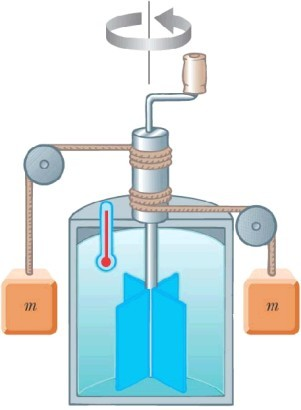
\includegraphics[width=0.5\textwidth]{mulinello_joule.jpg}
    \caption{Il Mulinello di Joule}
\end{figure}
Questo esperimento porta ad un aumento di temperatura nell'acqua che risulta proporzionale al lavoro svolto, così come l'aumento di temperatura era proporzionale al calore fornito al sistema. Ciò significa che calore e lavoro sono due grandezze proporzionali secondo una costante di proporzionalità che vale (se Q è misurato in calorie ed L in joule):
\[\frac{Q}{L}\approx4,186\]
Pertanto lavoro e calore rappresentano due diversi modi di trasmettere energia.  
\paragraph{Trasformazioni di Fase}
Le trasformazioni di Fase sono trasformazioni di un sistema termodinamico \textbf{isoterme} (ossia avvengono a temperatura costante). Inoltre, fissata la pressione, il calore necessario per compiere una tale trasformazione su un corpo è direttamente proporzionale alla sua massa. Vale pertanto:
\[\lambda=\frac{Q}{m}\]
In generale tuttavia questo valore non è costante, e può essere scritto come derivata del calore rispetto alla massa:
\[\lambda=\dv{Q}{m}\]
Ossia il calore necessario $\delta Q$ a compiere una trasformazione di fase su un quantità di massa $\dif m$.
\section{Il Primo Principio}
\paragraph{Il Lavoro Termodinamico}
Per definire la quantità di lavoro $\delta L$ compiuta (o subita) da un corpo durante una certa trasformazione consideriamo un gas all'interno di un contenitore cilindrico la cui base superiore è un pistone mobile, allora si raggiungerà l'equilibrio quando:
\[\delta L+\F^{(e)}\cdot\dif\r=0\iff \delta L=-\F^{(e)}\cdot\dif\r=p^{(e)}A\dif h=p^{(e)}\dif h\]
Dove $\F^{(e)}$ è la risultante delle forze esterna, $\dif\r$ è lo spostamento infinitesimo del pistone, A la superficie del pistone, $p^{(e)}$ la pressione esterna risultante e $\dif V$ la variazione di volume infinitesimo.

\subsection{Le Trasformazioni Termodinamiche}
Parliamo di \textbf{trasformazione termodinamica} da uno stato iniziale ad uno stato finale un passaggio da un equilibrio termodinamico ad un altro. In generale tale trasformazione risulta impossibile da rappresentare su un piano termodinamico p-V in quanto solo agli equilibri le grandezze termodinamiche sono ben definite. Possiamo però rappresentare come segue una trasformazione di questo tipo:
\begin{figure}[H]
    \centering
    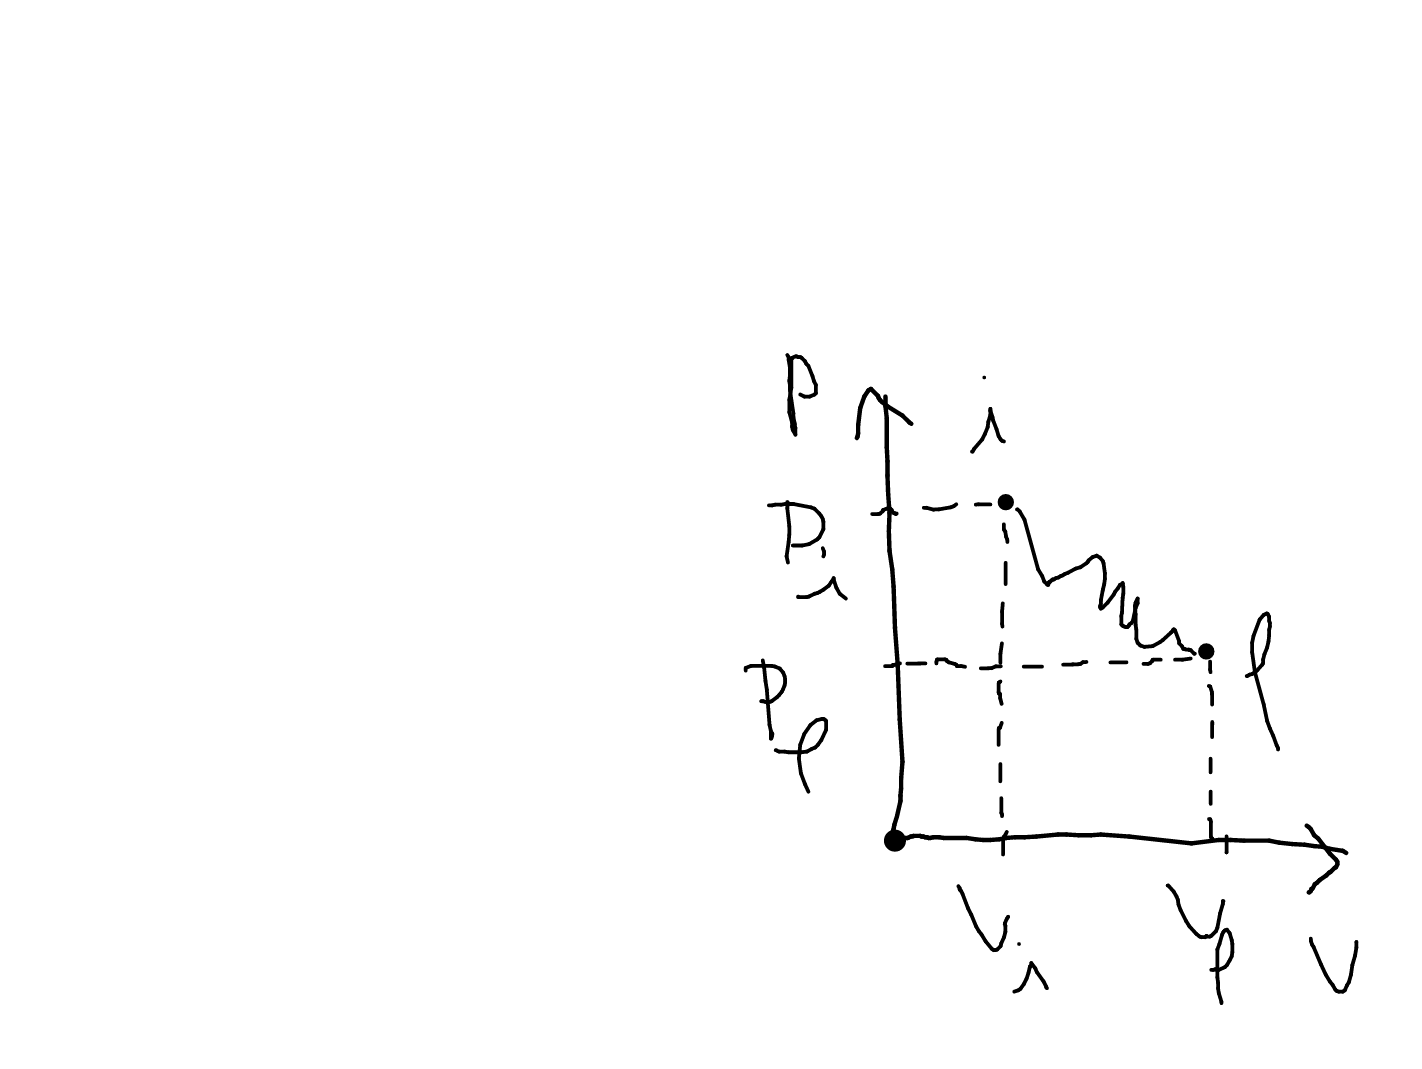
\includegraphics[width=0.5\textwidth]{TrasformazioneIrreversibile.png}
    \caption{Esempio di Trasformazione Termodinamica}
    \label{TrasfIrrev}
\end{figure}

\paragraph{Formulazione del Primo Principio}
Il \textbf{Primo Principio della Termodinamica} si può enunciare come segue:
\begin{defn}
Se un sistema compie una trasformazione dallo stato termodinamico A a B, scambiando calore e lavoro con l'ambiente, la quantità $Q-L$ è indipendente dalla trasformazione. 
\end{defn}
\begin{equation}
    \boxed{Q-L=\Delta U}
\end{equation}
Questa equazione è particolarmente significativa in quanto afferma l'esistenza di una funzione di stato U, detta \textbf{energia interna}, tale che $\Delta U=U(B)-U(A)=Q-L$. Il primo principio da solo non stabilisce limite sulla "\textit{riutilizzabilità}" dell'energia interna, ma come stabilito dal secondo principio della termodinamica, esistono limiti. \\
Inoltre notiamo che tutte le grandezze coinvolte sono misurate \textit{dall'esterno}, quindi variazioni di temperatura, volumi, pressioni e masse all'equilibrio che permettono di descrivere il comportamento del sistema termodinamico. Così facendo ha senso fissare la convenzione per cui lavoro e calore ceduti dall'esterno al sistema sono positivi, mentre lavoro e calore ceduti dal sistema all'ambiente sono negativi. 
\paragraph{Trasformazioni Infinitesime}
Queste sono trasformazioni ottenute per infinitesime quantità di calore e lavoro scambiati con l'esterno da un sistema (a cui corrispondono infinitesima variazioni di pressione, volume e temperatura). Studiando un sistema con varianza 2 otteniamo il primo principio per quantità infinitesime:
\[\delta Q-\delta L=\dif U\]
Notiamo che Q ed L sono \textbf{forme differenziali} in quanto non sono funzioni di stato, diversamente dall'energia interna.\\ Calcoliamo la quantità di calore infinitesima fornita utilizzando la definizione di lavoro e la proprietà di differenziale esatto di energia interna:
\[\delta Q=\dif U+\delta L=\left(\pdv{U}{t}\right)_V\dif t+\left(\pdv{U}{V}\right)_t\dif V+p^{(e)}\dif V\]
Otteniamo quindi la seguente \textbf{formula del calore} per trasformazioni infinitesime:
\begin{equation}
\boxed{\delta Q=\left(\pdv{U}{t}\right)_V\dif t+\left[\left(\pdv{U}{V}\right)_t+p^{(e)}\right]\dif V}
\end{equation}
Per una trasformazione infinitesima \textbf{isocora} si riduce a:
\[\delta Q=\left(\pdv{U}{t}\right)_V\dif t\]
Ma per definizione di calore specifico molare:
\[\dv{Q}{t}=\left(\pdv{U}{t}\right)_V=n\overline{c}_V\then \boxed{\delta Q=n\overline{c}_V\dif t+\left[\left(\pdv{U}{V}\right)_t+p^{(e)}\right]\dif V}\]
Siccome l'energia interna è una funzione di stato, questa espressione è valida per ogni trasformazione infinitesima.
Per i liquidi e i solidi, considerati incompressibili possiamo porre $\dif V=0$, mentre il calore specifico molare è uguale sia a pressione che a volume costante. Pertanto il calore si riduce all'espressione della trasformazione isocora per liquidi e solidi.
\subsection{Le Leggi dei Gas Ideali}
Per quanto riguarda i gas il comportamento si può generalizzare ad ogni gas nel caso in cui essi siano \textbf{rarefatti}, ossia poco densi e ad alta temperatura. In particolare valgono le seguenti leggi:
\begin{enumerate}
    \item La \textbf{Prima Legge di Gay-Lussac} \[V=V_0(1+\alpha t)\]
    Dove $\alpha$ è una costante che vale $\frac{1}{273,16\si{\degreeCelsius}}$ per gas rarefatti, $V_0$ è il volume a pressione atmosferica e $0\si{\degreeCelsius}$ e la pressione è costante.
    \item La \textbf{Seconda Legge di Gay-Lussac} \[p=p_0(1+\alpha t)\]
    Con volume costante e dove $p_0$ è la costante atmosferica.
    \item La \textbf{Legge di Boyle} \[pV=p_0V_0\]
    Che è valida a temperatura costante.
\end{enumerate}
Da queste leggi possiamo ricavare l'\textbf{equazione di stato} per i gas ideali. Immaginiamo di sottoporre il gas ad una trasformazione isobara, vale allora la prima legge di Gay-Lussac:
\[V_1=V_0(1+\alpha t)\]
Sottoponiamola poi ad una trasformazione isoterma, in modo che sia valida la legge di Boyle:
\[pV=p_0V_1=p_0V_0(1+\alpha t)\]
Esplicitando $V_0$ come prodotto del numero di moli e del volume molare otteniamo (abbiamo implicitamente usato la \textbf{Legge di Avogadro} nell'affermare che tutti i gas rarefatti hanno lo stesso volume molare):
\[pV=p_0n\overline{v}_0\alpha \left(t+\frac{1}{\alpha}\right)\]
Definiamo quindi una nuova scala di temperatura, detta \textbf{scala di Kelvin} tale che $\theta=(t+273,16)K$ e poi definiamo la \textbf{costante universale dei gas} come $R=p_0\overline{v}_0\alpha$ ottenendo infine:
\begin{equation}
\boxed{pV=nR\theta}
\end{equation}
Ossia l'equazione di stato dei gas perfetti.

\subsection{L'Energia Interna dei Gas}
Vogliamo ora dimostrare che l'energia interna di un gas è funzione unicamente delle temperatura (come variabile termodinamica). Utilizziamo come esempio la \textbf{seconda esperienza di Joule}.
\begin{figure}[H]
    \centering
    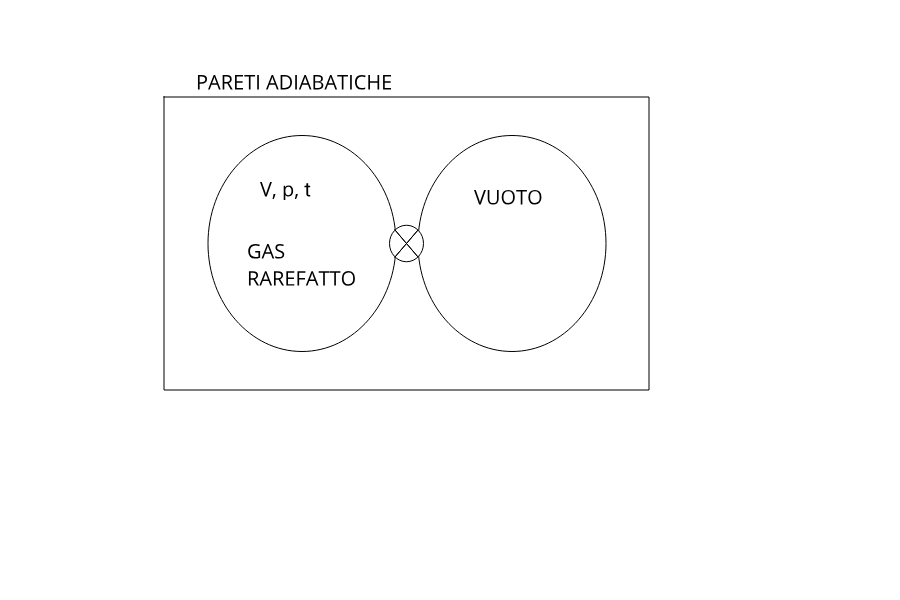
\includegraphics[width=0.5\textwidth]{SecondoJoule.png}
    \caption{Stato Iniziale del Secondo Esperimento di Joule}
    \label{SecondoJoule}
\end{figure}
Costruiamo un sistema isolato con delle pareti adiabatiche dall'esterno e in contatto con un altro contenitore tramite una valvola. Immaginiamo di \textbf{bruscamente} aprire questa valvola, otterremo che all'equilibrio il gas occupa tutto il volume. Inoltre si può misurare che all'equilibrio la temperatura risulta invariata:\\
\begin{center}
\begin{tabular}{c|c|c|c}
    INIZIO & $V_i=V_1$ & $p_i=p_0$ & $t_i=t_1$ \\
    \hline
    FINE & $V_f=V_1+V_2$ & // & $t_f=t_1$
\end{tabular} 
\end{center}
Ripetendo l'esperimento a densità molare decrescente otteniamo il seguente grafico:\\
\begin{center}
\begin{tikzpicture}
\begin{axis}[
    axis lines = left,
    xlabel = $\frac{n}{V_i}$,
    ylabel = {$t_i-t_f$},
]
\addplot [
    domain=0:10, 
    samples=10, 
    color=red,
]
{x*0.3};
\end{axis}
\end{tikzpicture}
\end{center}
Ossia otteniamo una funzione che tende a 0 al calare della densità molare. Osserviamo inoltre che essendo le pareti adiabatiche e fisse, esse isolano il sistema sia meccanicamente che termicamente in modo che non ci siano scambi di calore nè l'ambiente possa compiere lavoro sul sistema (o viceversa), quindi la variazione di energia interna è nulla:
\[\Delta U=Q-L=0\then U_i=U_f\]
Scelte t e V come variabili termodinamiche del sistema allora vale:
\[U(t_1,V_1)=U(t_1,V_1+V_2)=U(t_1,yV_1)\]
Ossia il volume a temperatura costante varia linearmente, quindi:
\[\pdv{U}{V}=0\then U=U(t)=U(\theta)\]
Ossia l'energia interna è una \textbf{funzione di stato} che dipende unicamente dalla \textit{temperatura}.\\
Pertanto un gas ideale è descritto termodinamicamente dall'equazione di stato e della funzione energia interna:
\begin{equation}
\begin{cases}
pV=nR\theta\\
U=U(\theta)
\end{cases}
\end{equation}
Per un gas ideale vale allora la seguente espressione di calore ed energia interna:
\begin{equation}
\boxed{(\delta Q)_V=n\overline{c}_V\dif\theta=\dif U}\then \boxed{U(\theta)=\int n\overline{c}_V(\theta)\dif\theta+cost}
\end{equation}
Queste considerazioni (fatte in questa situazione) sono tuttavia valide in ogni trasformazione termodinamica, in quanto l'energia interna è una funzione di stato. Mentre l'espressione generale del calore è:
\[\delta Q=n\overline{c}_V\dif\theta+p^{(e)}\dif V\]

\paragraph{I Calori Specifici dei Gas Ideali}
Il calore specifico molare a volume costante per i gas si comporta (sommariamente) come in figura, dove i monoatomici hanno $\overline{c}_V$ costante, i biatomici hanno $\overline{c}_V$ a "scaletti" a cui corrisponde microscopicamente lo "sblocco" dei gradi di libertà delle molecole e infini i poliatomici hanno andamenti altamente complicati, la cui curva tende a diventare più \textit{liscia} all'aumentare degli atomi componenti. Generalmente la fascia considerata è quella in cui i gas biatomici hanno $\overline{c}_V=\frac{5}{2}R$ e i monoatomici hanno $\overline{c}_V=\frac{3}{2}R$.\\
Vale inoltre la \textbf{legge di Mayer} che stabilisce che:
\begin{equation}
\boxed{\overline{c}_p-\overline{c}_V=R}
\end{equation}

\subsection{Le Trasformazioni Reversibili}
\begin{defn}[Trasformazione Quasistatica]
Si definisce trasformazione \textbf{quasistatica} una trasformazione ottenuta tramite somma di trasformazioni infinitesime. Praticamente ciò implica che una trasformazione quasistatica si può rappresentare sul piano p-V (detto \textbf{piano di Clapeyron}):
\[\int_A^B\delta Q-\int_A^B\delta L=\int_A^B\dif U\]
In questo caso sono ben definite tutte le grandezze termodinamiche per ogni variazione, quindi per il calcolo del lavoro si può utilizzare la pressione del gas (uguale a quella esterna). 
\end{defn}
\begin{defn}[Trasformazione Reversibile]
Una trasformazione quasistatica si dice reversibile se può essere ripetuta in senso inverso seguendo gli stessi stati di equilibrio punto per punto. 
\end{defn}
Tra le più comuni trasformazioni reversibili individuiamo le seguenti quattro:
\begin{figure}[H]
    \centering
    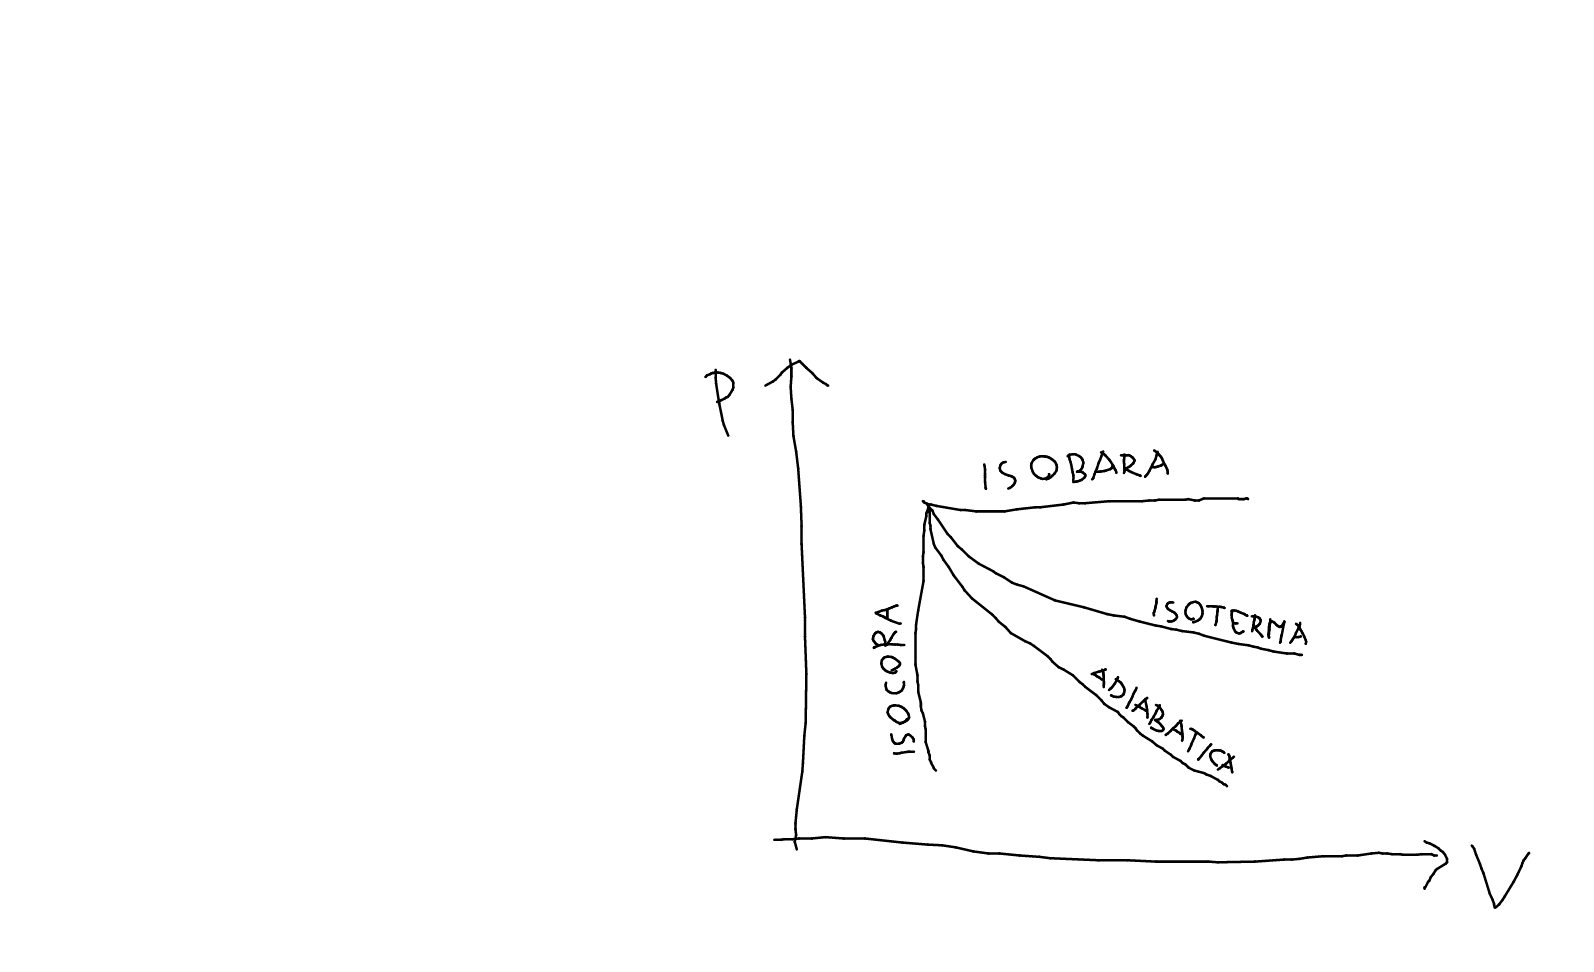
\includegraphics[width=0.6\textwidth]{TrasformazioniReversibili.png}
    \caption{Le Maggiori Trasformazioni Reversibili }
    \label{TrasfRevers}
\end{figure}
\paragraph{Trasformazione Adiabatica Reversibile} Considerando un'adiabatica reversibile possiamo applicare il primo principio per le trasformazioni infinitesime e poi integrando tra uno stato A e B:
\[\delta Q=\dif U+\delta L=n\overline{c}_V\dif\theta+p\dif V=0\then \overline{c}_V\frac{\dif\theta}{\theta}+R\frac{\dif V}{V}=0\then \overline{c}_V\ln\frac{\theta_B}{\theta_A}+R\ln\frac{V_B}{V_A}=0\]
Definita la costante $\gamma=\frac{\overline{c}_p}{\overline{c}_V}$ allora possiamo esplicitare come segue:
\begin{equation}
\begin{split}
    \ln\frac{\theta_B}{\theta_A}+\frac{R}{\overline{c}_V}\ln\frac{V_B}{V_A}&=0\\
    \ln\frac{\theta_B}{\theta_A}+(\gamma-1)\ln\frac{V_B}{V_A}&=0\\
    \ln\frac{\theta_B}{\theta_A}+\ln\left(\frac{V_B}{V_A}\right)^{\gamma-1}&=0\\
    \ln\left[\frac{\theta_B}{\theta_A}\left(\frac{V_B}{V_A}\right)^{\gamma-1}\right]&=0\\
\end{split}
\end{equation}
Per le proprietà dei logaritmi otteniamo:
\[\frac{\theta_B}{\theta_A}\left(\frac{V_B}{V_A}\right)^{\gamma-1}=1\then \theta_BV_B^{\gamma-1}=\theta_AV_A^{\gamma-1}\]
Ossia:
\begin{equation}
\boxed{\theta V^{\gamma-1}=cost}
\end{equation}
Utilizzando l'equazione di stato dei gas ideali possiamo anche ottenere le seguenti espressioni:
\[pV^{\gamma}=cost\quad Tp^{\frac{1-\gamma}{\gamma}}\]



\section{Secondo Principio della Termodinamica}
\begin{defn}[Sorgente]
Un sistema che mantiene la propria temperatura costante.
\end{defn}
\begin{defn}[Macchina Termica]
Una macchina termica è un dispositivo capace di scambiare calore (con due o più sorgenti) e lavoro (con l'ambiente). 
\end{defn}
\begin{defn}[Enunciato di Clausius]
Non è possibile effettuare una trasformazione termodinamica il cui unico risultato sia il trasferimento di una quantità finita di calore da una sorgente fredda ad una calda.
\end{defn}
\begin{defn}[Enunciato di Kelvin-Planck]
Non è possibile realizzare una trasformazione termodinamica che abbia come unico risultato la trasformazione in lavoro del calore fornito da una sorgente.
\end{defn}
\begin{defn}[Rendimento]
Il rendimento di una macchina termica si definisce come:
\[\eta=\frac{L}{Q_A}=1+\frac{Q_B}{Q_A}\]
\end{defn}
\note L'enunciato di Kelvin equivale a dire che il rendimento di una macchina termica è minore di 1.\\
Dimostriamo ora l'equivalenza di questi due enunciati.
\begin{thm}[Clausius Implica Kelvin]
Supponiamo per assurdo che l'enunciato di Kelvin sia falso. Possiamo quindi costruire una macchina termica K che converte interamente lavoro in calore (ad esempio il Mulinello di Joule). Introduciamo poi un'altra macchina frigorifera $M_f$ su cui la prima macchina compie lavoro in modo che assorba calore dalla prima sorgente e ceda calore ad un'altra sorgente, più calda. L'effetto totale è quindi che la sorgente a temperatura fredda ha ceduto calore ad una sorgente a temperatura più alta. Ciò implica che l'enunciato di Clausius sia falso, abbiamo quindi raggiunto l'assurdo.
\begin{figure}[H]
    \centering
    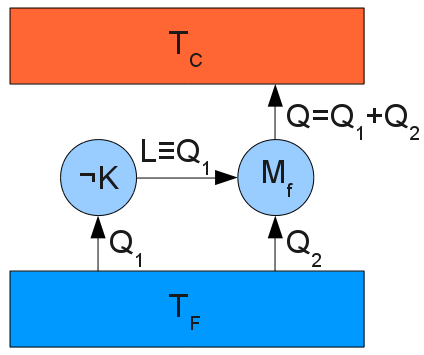
\includegraphics[width=0.5\textwidth]{Kelvin_dimostrazione_assurdo.png}
    \caption{Schema del Sistema Costruito}
    \label{ClausiusKelvin}
\end{figure}
\end{thm}
\begin{thm}[Kelvin Implica Clausius]
Supponiamo per assurdo che l'enunciato di Clausius sia falso. Costruiamo quindi una macchina termica C che assorbe una quantità di calore Q da una sorgente fredda e lo cede ad una calda (in quanto Clausius è falso) come unico risultato. Introduciamo quindi una macchina termica $M_t$ che assorbe una quantità di calore Q' compiendo lavoro L in modo che la quantità di calore ceduta alla sorgente a temperatura minore sia la stessa di quella assorbita dalla macchina C. Abbiamo quindi costruito una trasformazione il cui unico risultato sia quello di convertire calore in lavoro (l'effetto totale è di non coinvolgere la sorgente a temperatura fredda), quindi l'enunciato di Kelvin è falso. Abbiamo raggiunto l'assurdo, come volevasi dimostrare. 
\begin{figure}[H]
    \centering
    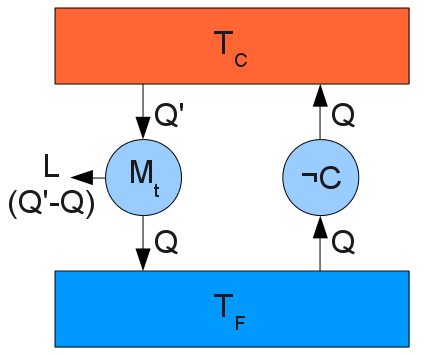
\includegraphics[width=0.5\textwidth]{Clausius_dimostrazione_assurdo.png}
    \caption{Schema del Sistema Costruito}
    \label{KelvinClausius}
\end{figure}
\end{thm}

\paragraph{Teorema di Carnot}
\begin{thm}[Teorema di Carnot]
Ogni macchina reversibile che lavoro tra due sorgenti alla stessa temperatura ha lo stesso rendimento. Qualsiasi altra macchina che lavori tra queste sorgenti ha rendimento non maggiore. Il risultato è indipendente dalle trasformazioni del ciclo. 
\end{thm}
\begin{proof}
Costruiamo due macchine termiche X ed R che lavorano tra le stesse sorgenti e tali da compiere lo stesso lavoro L, assorbendo rispettivamente una quantità di calore $Q_1$ e $Q_1'$ e cedendo una quantità di calore $Q_2$ e $Q_2'$ alla sorgente calda e fredda rispettivamente. 
\begin{figure}[H]
    \centering
    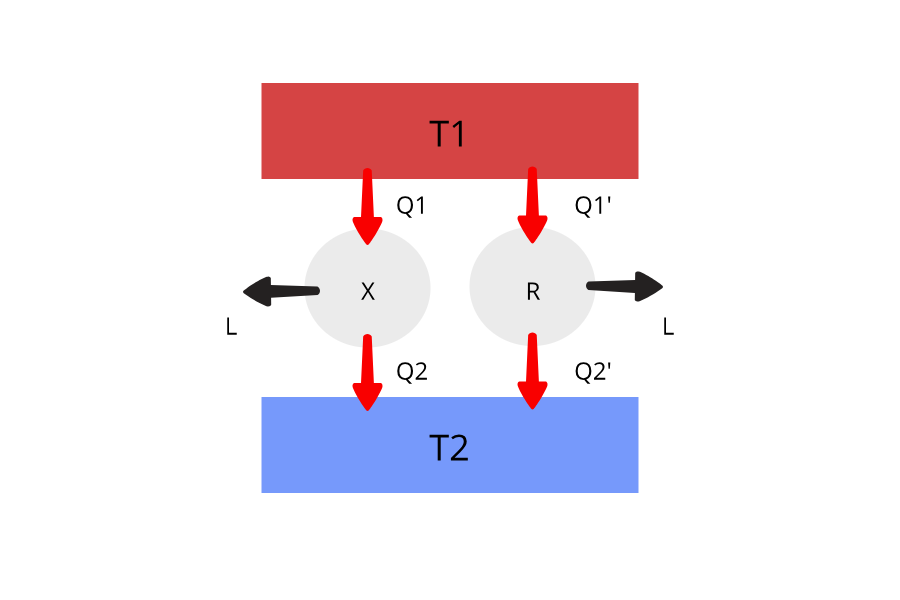
\includegraphics[width=0.7\textwidth]{TeoremaCarnot1.png}
    \label{TeoremaCarnot1}
\end{figure}
Supponendo che la macchina \textbf{R} sia reversibile, utilizziamo il lavoro della macchina \textbf{X} per invertire il ciclo della macchina R in modo che diventi refrigerante (stavolta i calore scambiati da R sono invertiti di segno).
\begin{figure}[H]
    \centering
    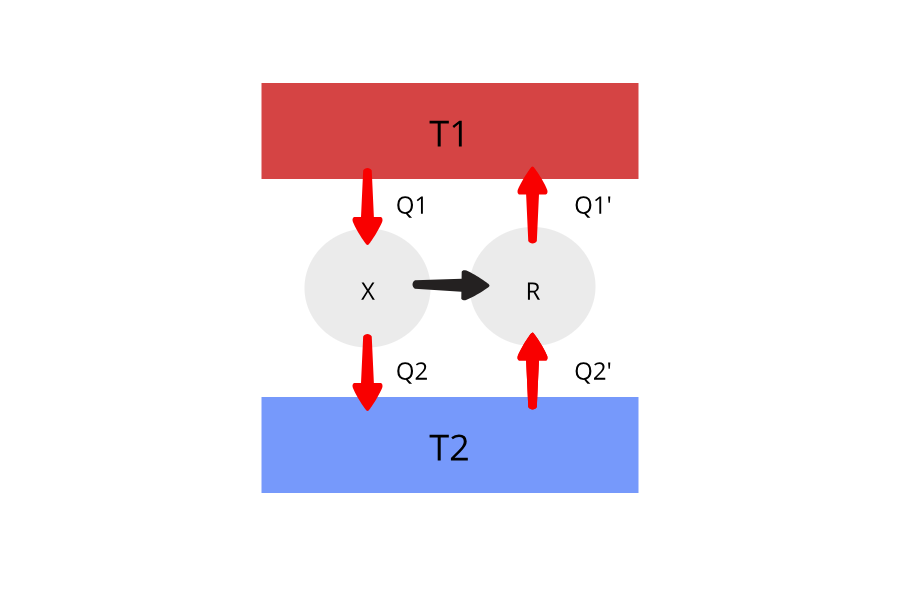
\includegraphics[width=0.7\textwidth]{TeoremaCarnot2.png}
    \label{TeoremaCarnot2}
\end{figure}

Per l'enunciato di Clausius deve risultare che la quantità di calore totale ceduta dalla sorgente calda è maggiore di quella ceduta da quella fredda, quindi otteniamo:
\[\abs{Q_1}\geq\abs{Q_1'}\then \frac{Q_1'}{Q_1}\leq 1\]
Calcoliamo quindi i rendimenti delle due macchine:
\begin{equation}
\eta_X=\frac{L}{Q_1}\quad\eta_R=\frac{L}{Q_1'}\then \eta_X\abs{Q_1}=\eta_R\abs{Q_1'}\then \eta_X=\eta_R\frac{\abs{
Q_1'}}{\abs{Q_1}} \leq \eta_R\then\boxed{\eta_X\leq\eta_R}
\end{equation}

Abbiamo dimostrato la \textbf{prima parte della tesi}. Dimostriamo ora la seconda.
Supponiamo che X sia reversibile, allora possiamo invertire i ragionamenti fatti in modo da ottenere:
\[\eta_X\geq\eta_R\]
Ma allora l'unica possibilità è che i due rendimenti coincidano:
\begin{equation}
\boxed{\eta_X=\eta_R}
\end{equation}
\end{proof}
\note Il risultato è indipendente dalle trasformazioni del ciclo in quanto l'unica proprietà che abbiamo assunto dalle macchine è che una fosse reversibile.\\
\note L'uguaglianza come caso limite nel primo risultato è nel caso in cui entrambe le macchine siano irreversibili oppure nel caso $Q_1=Q_1'=0\iff L=0$ ossia la macchina sta operando alcuna trasformazione.

\paragraph{Definizione di Temperatura Assoluta}
Dimostrato il Teorema di Carnot siamo in grado di dare una definizione assoluta di temperatura utilizzando il risultato per cui ogni macchina reversibile che opera tra certe due sorgenti ha lo stesso rendimento, ciò implica che il rendimento di una macchina reversibile R è funzione delle due temperature:
\[\eta=\eta(t_1,t_2)=1+\frac{Q_2}{Q_1}\]
Definiamo quindi la funzione g come segue:
\[g(t_1,t_2)=1-\eta(t_1,t_2)=\frac{\abs{Q_2}}{\abs{Q_1}}\]
Costruiamo poi il seguente sistema formato da tre sorgenti e due macchine termiche nel modo seguente (dove $\abs{Q_2}=\abs{Q_2'}$):
\begin{figure}[H]
    \centering
    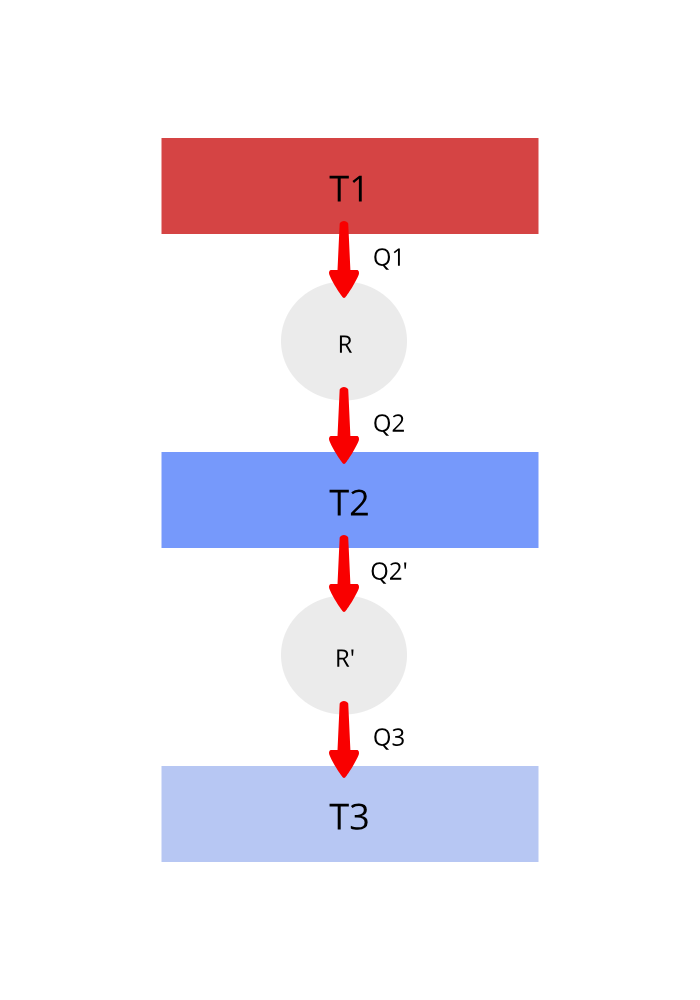
\includegraphics[width=0.4\textwidth]{TemperaturaAssoluta.png}
    \label{TemperauraAssoluta}
\end{figure}
Corto-circuitiamo le due macchine termiche in modo da ottenere un'unica macchina termica reversibile che lavora tra la sorgente a temperatura $t_1$ e quella a temperatura $t_3$ scambiando rispettivamente una quantità di calore $Q_1$ e $Q_3$.
\begin{figure}[H]
    \centering
    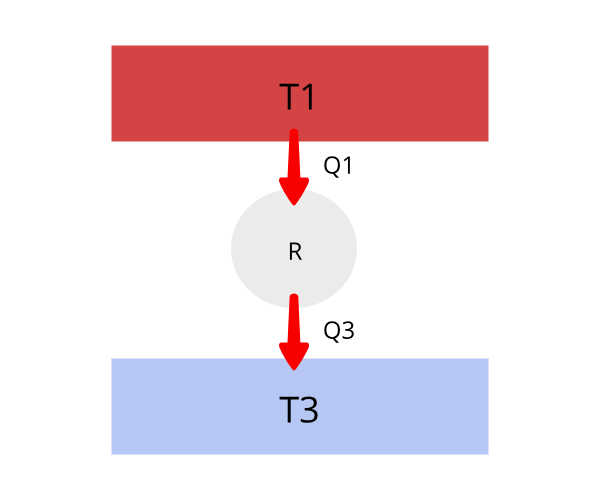
\includegraphics[width=0.5\textwidth]{TempAss.png}
\end{figure}
La funzione g di questa macchina termica è:
\[g(t_1,t_3)=\frac{\abs{Q_3}}{\abs{Q_1}}\]
Mentre delle due macchine singolarmente:
\[g(t_1,t_2)=\frac{\abs{Q_2}}{\abs{Q_1}}\quad g(t_2,t_3)=\frac{\abs{Q_3}}{\abs{Q_2'}}\]
Allora vale la relazione:
\[g(t_1,t_3)=g(t_1,t_2)\cdot g(t_2,t_3)\quad\forall t_2\]
Ciò significa che g è una funzione indipendente da $t_2$. Possiamo scriverla quindi come rapporto di una funzione f applicata in $t_3$ e applicata in $t_2$:
\[g(t_1,t_3)=\frac{f(t_3)}{f(t_1)}\]
Chiamiamo questa funzione f(t) \textbf{temperatura termodinamica assoluta} e poniamo $g(P.T.)=T_{pt}=273,16K$ ossia poniamo la temperatura assoluta del punto triplo (un punto termodinamico ben definito) dell'acqua uguale a $273,16K$. Possiamo quindi misurare la temperatura $T_x$ di una sorgente misurando i calori scambiati con una macchina che lavoro tra $T_{pt}$ e $T_x$:
\[T_x=T_{pt}\frac{\abs{Q_x}}{\abs{Q_{pt}}}\]
Ossia il II Principio fornisce un metodo di misurazione \textbf{assoluta} di temperatura.

\note La scala assoluta e la scala Kelvin coincidono in quanto:
\[\frac{T_x}{T_{pt}}=\frac{\theta_x}{\theta_{pt}}=\frac{\theta_x}{T_{pt}}\iff T_x=\theta_x\]

\subsection{Il Ciclo di Carnot}
Il Ciclo di Carnot è un ciclo composto da quattro trasformazioni reversibili:
\begin{enumerate}
    \item AB \textbf{Espansione Isoterma} ($Q>0$)
    \item BC \textbf{Espansione Adiabatica} ($Q=0$)
    \item CD \textbf{Compressione Isoterma} ($Q<0$)
    \item DA \textbf{Compressione Adiabatica} ($Q=0$)
\end{enumerate}
\begin{figure}[H]
    \centering
    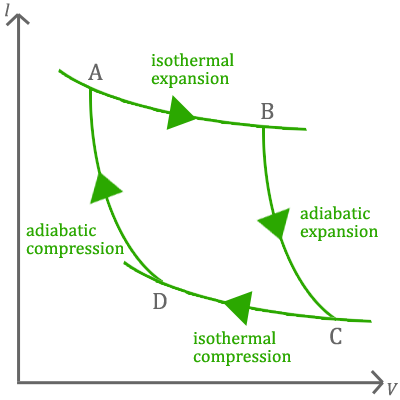
\includegraphics[width=0.6\textwidth]{CicloCarnot.png}
    \caption{Il Ciclo di Carnot}
    \label{CicloCarnot}
\end{figure}
Si può dimostrare che questa è l'unica trasformazione ciclica (percorsa nel senso in figura, tale che la macchina si comporti da macchina termica e \textit{compia} lavoro) che avviene solo tra due sorgenti (e quindi \textbf{due temperature}. Studiamo ora quanto vale il rendimento di una macchina (detta \textbf{macchina di Carnot}) che compie questo ciclo. \\
Durante l'espansione isoterma AB il calore è assorbito dalla sorgente calda a temperatura $T_2$ (uguale al lavoro compiuto dal sistema) e vale:
\[Q_2=nRT_1\ln\frac{V_B}{V_A}\]
Durante l'espansione adiabatica BC vale la relazione tra volume e temperatura:
\[T_BV_B^{\gamma-1}=T_CV_C^{\gamma-1}\iff T_2V_B^{\gamma-1}=T_1V_C^{\gamma-1}\then \left(\frac{V_C}{V_B}\right)^{\gamma-1}=\frac{T_2}{T_1}\]
Durante la compressione isoterma CD il calore ceduto:
\[Q_1=nRT_1\ln\frac{V_D}{V_C}\]
E infine dalla compressione adiabatica DA otteniamo:
\[T_DV_D^{\gamma-1}=T_AV_A^{\gamma-1}\iff T_1V_D^{\gamma-1}=T_2V_A^{\gamma-1}\then \left(\frac{V_D}{V_A}\right)^{\gamma-1}=\frac{T_2}{T_1}\]
Combinando le due equazioni ottenute dalle adiabatiche:
\[\left(\frac{V_C}{V_B}\right)^{\gamma-1}=\frac{T_2}{T_1}=\left(\frac{V_D}{V_A}\right)^{\gamma-1}\then \frac{V_C}{V_B}=\frac{V_D}{V_A}\then\boxed{\frac{V_C}{V_D}=\frac{V_B}{V_A}}\]
Il rendimento del ciclo vale 
\begin{equation}
\begin{split}
    \eta&=1+\frac{Q_1}{Q_2}=1+\frac{nRT_B\ln\frac{V_D}{V_C}}{nRT_A\ln\frac{V_B}{V_A}}=\\
    &=1+\frac{T_1\ln\frac{V_D}{V_C}}{T_2\ln\frac{V_B}{V_A}}=1-\frac{T_1\ln\frac{V_C}{V_D}}{T_2\ln\frac{V_B}{V_A}}=\\
    &=\boxed{1-\frac{T_1}{T_2}}
\end{split}
\end{equation}
Come volevasi dimostrare, il rendimento di una macchina di Carnot dipende unicamente dalle temperature delle \textit{due} sorgenti tra cui opera. Inoltre usando il \textbf{Teorema di Carnot} ricaviamo che una macchina qualunque che opera tra due sorgenti (e quindi compie lo stesso tipo di trasformazioni, anche se irreversibili) ha un rendimento:
\[\eta\leq1-\frac{T_1}{T_2}\]
Inoltre per definizione di rendimento:
\[\eta=1+\frac{Q_1}{Q_2}\then \frac{Q_1}{Q_2}\leq -\frac{T_1}{T_2}\then \boxed{\frac{Q_1}{T_1}+\frac{Q_2}{T_2}}\]
Questa disuguaglianza è particolarmente importante in quanto rappresenta una prima forma di enunciato per il secondo principio della termodinamica, ma deve essere generalizzato in quanto per trovare questo risultato abbia supposto due ipotesi:
\begin{enumerate}
    \item La trasformazione operata dalla macchina è \textbf{ciclica}
    \item La macchina termica opera tra \textbf{due sorgenti}
\end{enumerate}


\section{L'Entropia}
\begin{thm}[Teorema di Clausius]
Il Teorema di Clausius permette di generalizzare il risultato ottenuto ad un numero arbitrario di sorgenti (fino ad una continuità di sorgenti). Consideriamo prima di tutto una macchina termica che compie una trasformazione ciclica tra n sorgenti:
\begin{figure}[H]
    \centering
    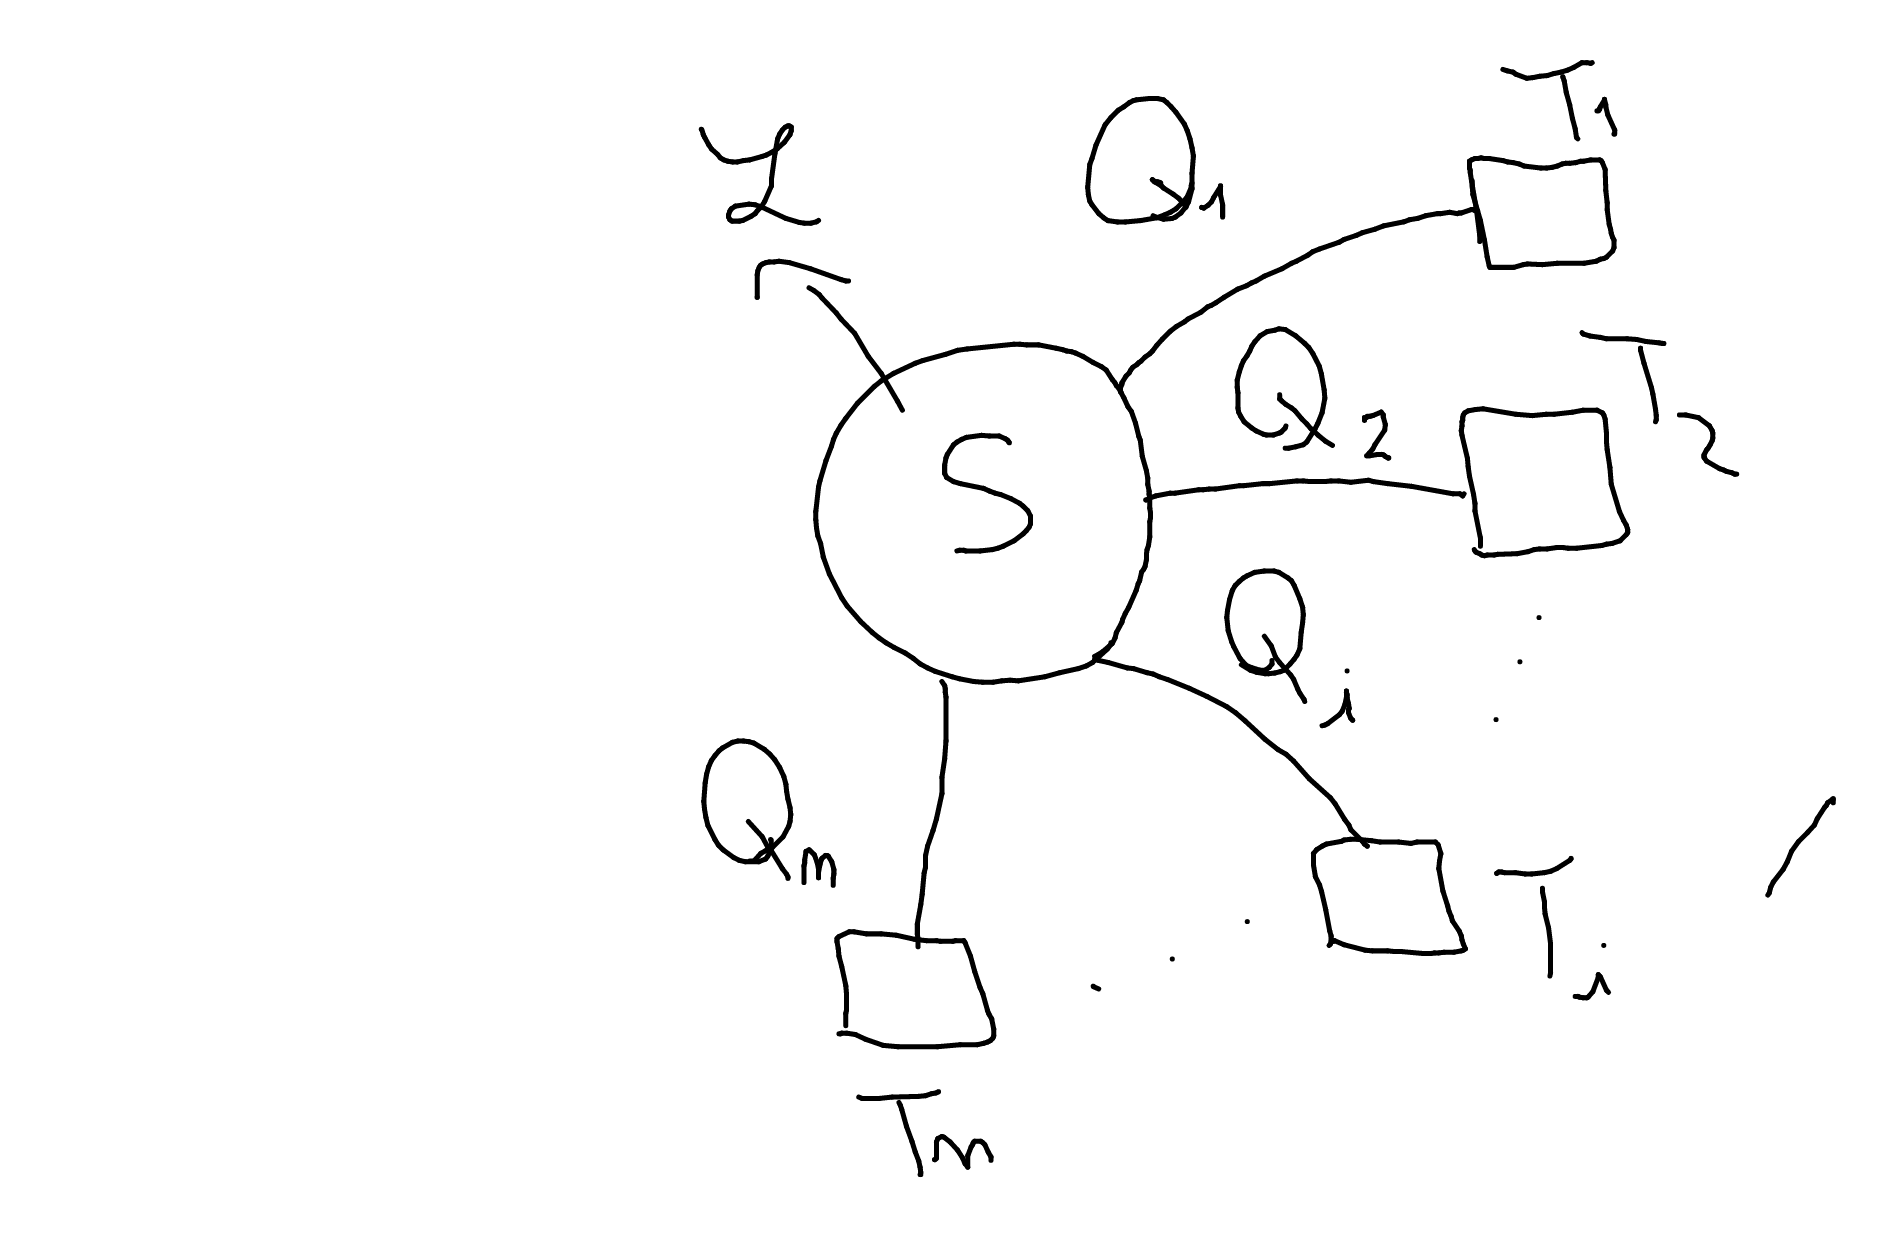
\includegraphics[width=0.5\textwidth]{TeoremaClausius1.png}
    \label{TeoremaClausius1}
\end{figure}
Introduciamo poi n macchine di Carnot reversibili che lavorano tra una sorgente a temperatura $T_0$ e l'i-esima sorgente a temperatura $T_i$, scambiando rispetivamente un certo calore $Q_{i0}$ con la prima sorgente e $-Q_i$ con le altre:
\begin{figure}[H]
    \centering
    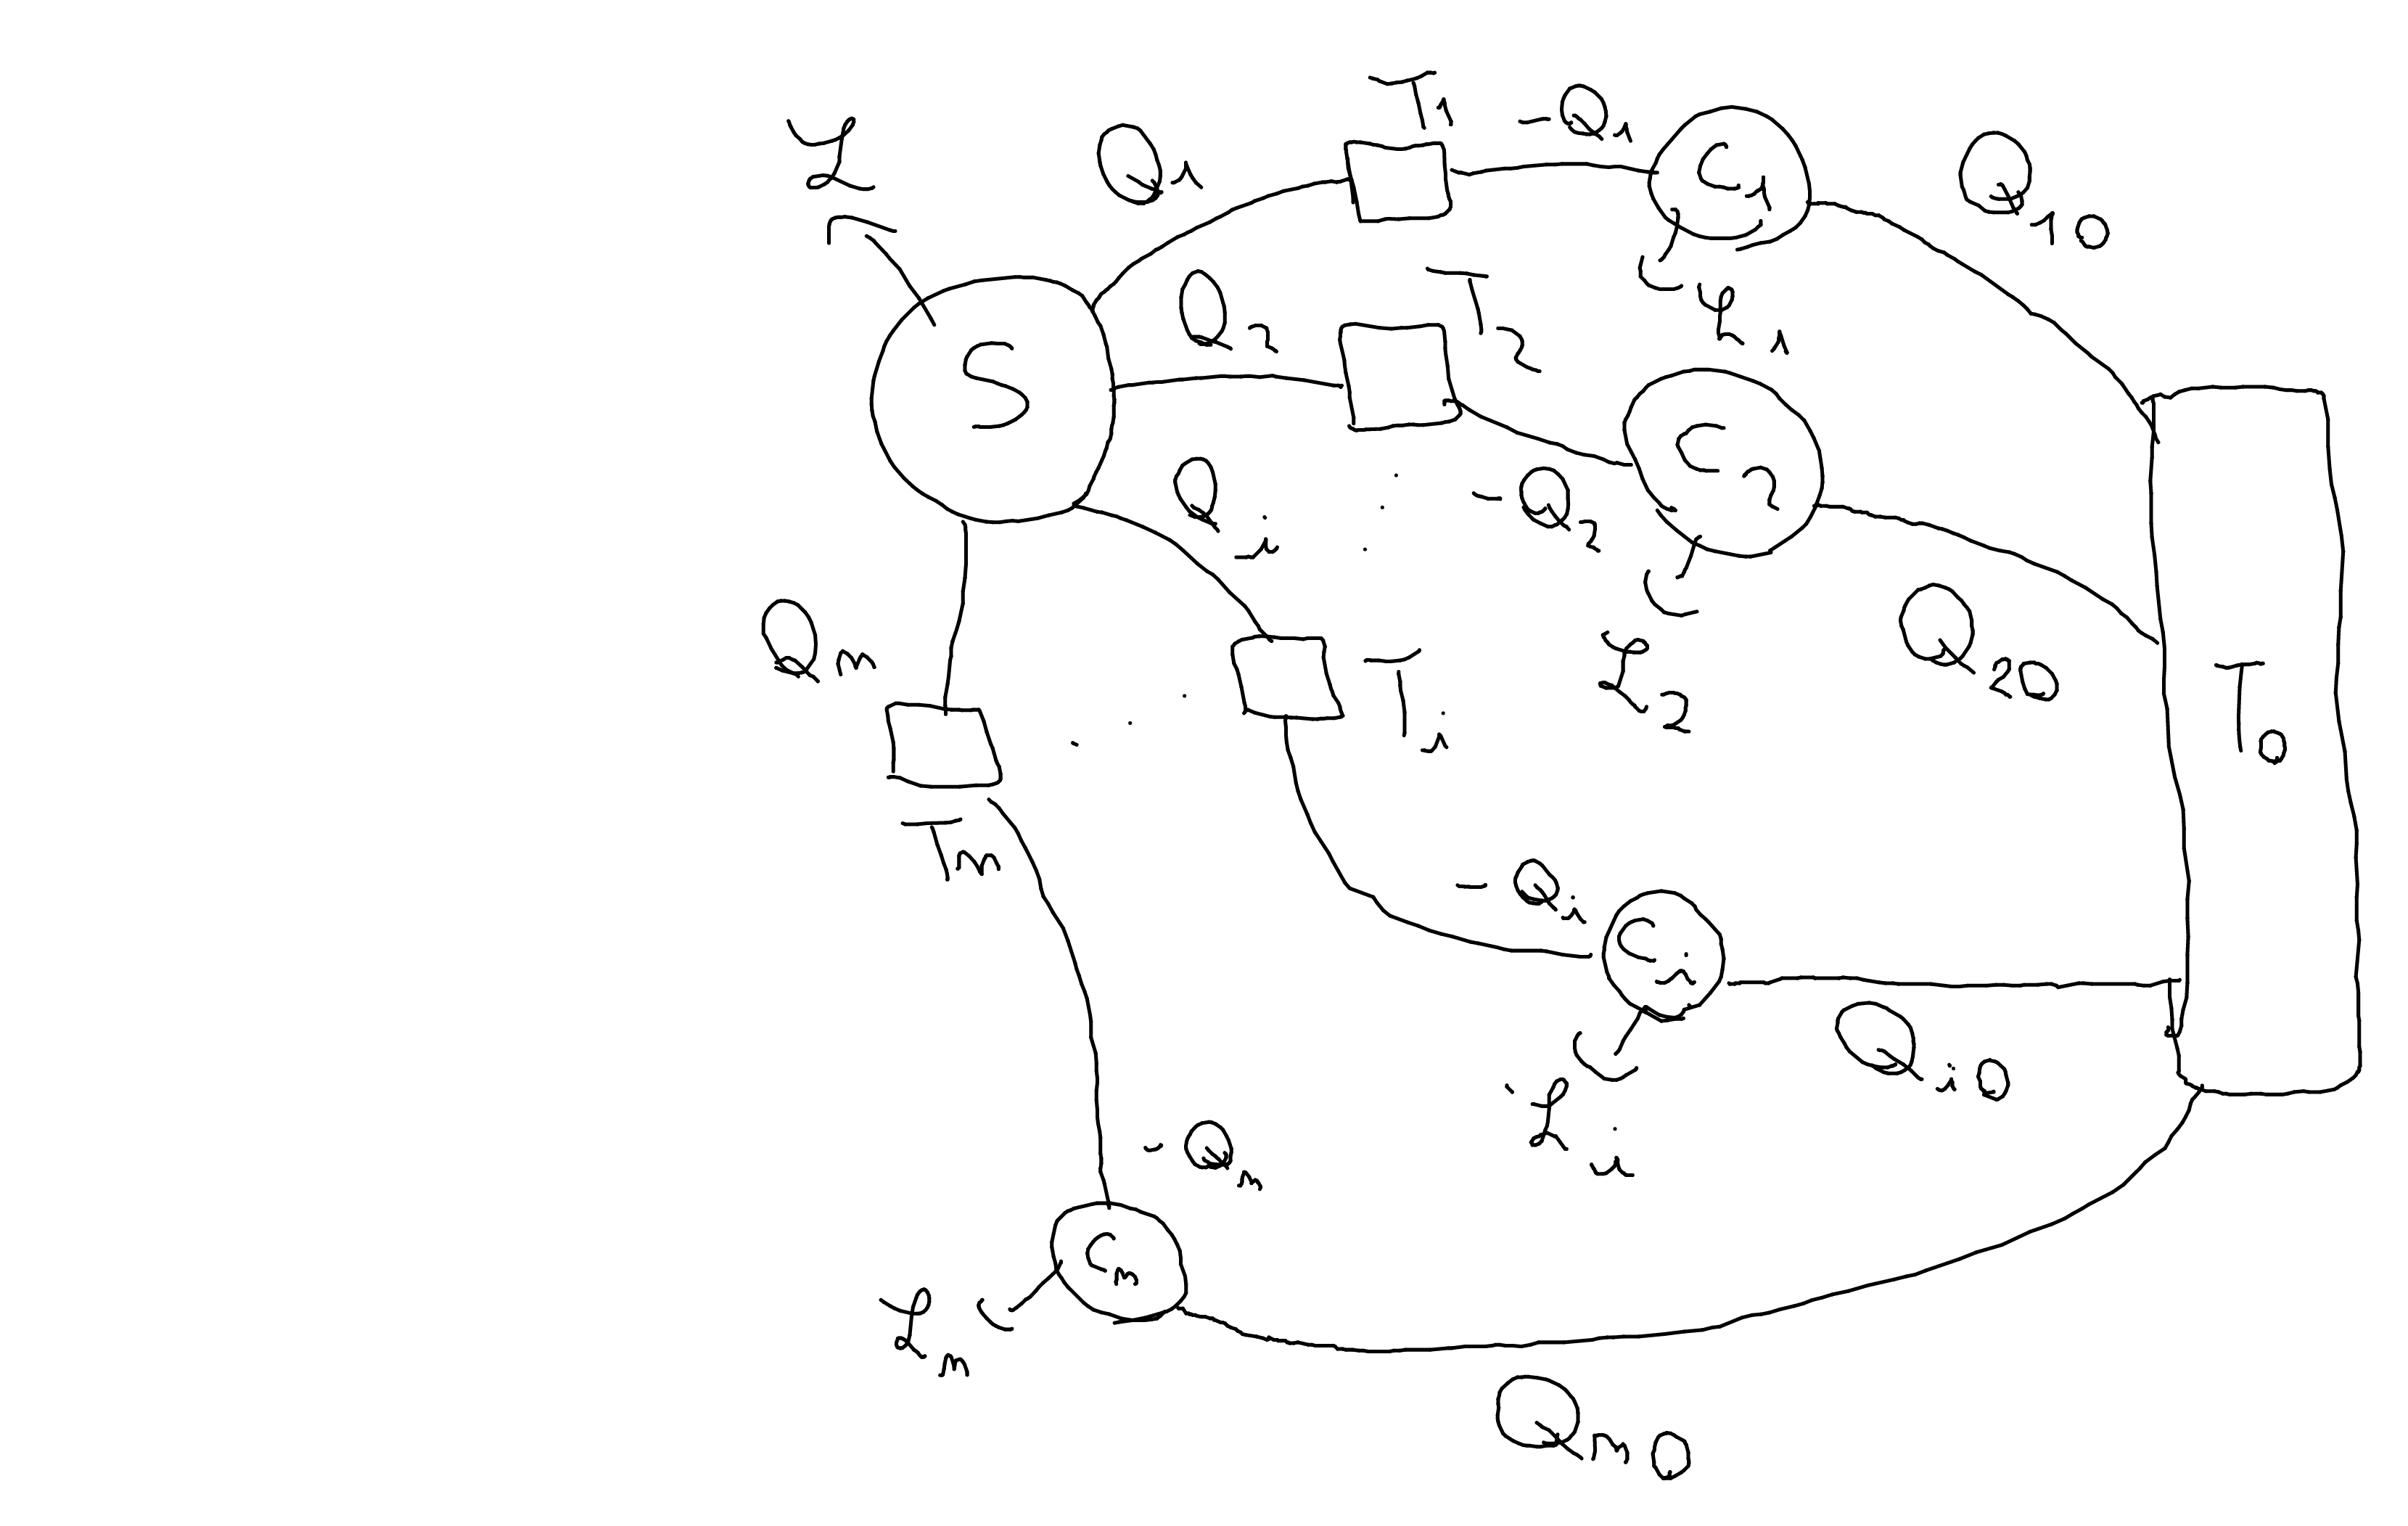
\includegraphics[width=0.5\textwidth]{TeoremaClausius2.png}
    \label{TeoremaClausius2}
\end{figure}
Abbiamo quindi effettivamente circuitato le sorgenti, ossia abbiamo costruito una nuova macchina termica che compie una trasformazione ciclica. Il calore totale scambiato dalla sorgente a temperatura $T_0$ deve essere tuttavia \textbf{ceduto} (o nullo) per l'enunciato di Kelvin (in quanto se fosse positivo l'unico risultato della trasformazione ciclica sarebbe il lavoro del sistema). Inoltre per il Teorema di Carnot applicato a ciascuna delle macchine termiche $C_i$ otteniamo:
\[-\frac{Q_i}{T_i}+\frac{Q_{i0}}{T_0}=0\then \frac{Q_{i0}}{T_0}=\frac{Q_i}{T_i}\]
Sommando sull'indice i otteniamo (detto $Q_0$ il calore totale ceduto dalla sorgente a temperatura $T_0$):
\[\sum_i\frac{Q_i}{T_i}=\sum_i\frac{Q_{i0}}{T_0}=\frac{Q_0}{T_0}\leq0\then \boxed{\frac{Q_i}{T_i}\leq0}\]
Questa relazione è nota come \textbf{disuguaglianza di Clausius}. Nel caso particolare in cui la macchina termia S compia una trasformazione ciclica reversibile otteniamo:
\begin{equation}
\boxed{\sum_i\frac{Q_i}{T_i}=0}
\end{equation}
Per un numero arbitrariamente grande di sorgenti (e quindi macchine di Carnot) otteniamo invece l'\textbf{integrale di Clausius} per una macchina reversibile:
\begin{equation}
    \boxed{\oint\frac{\delta Q}{T_{sorgente}}=\oint\frac{\delta Q}{T}=0}
\end{equation}
Che consiste nell'approssimare un qualunque ciclo con dei cicli di Carnot:
\begin{figure}[H]
    \centering
    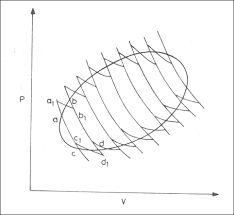
\includegraphics[width=0.3\textwidth]{IntegraleClausius.png}
    \caption{Approssimazione di un qualunque Ciclo Reversibile con dei Cicli di Carnot}
    \label{IntegraleClausius}
\end{figure}
In generale vale la disuguaglianza:
\begin{equation}
\boxed{\oint\frac{\delta Q}{T}\leq0}
\end{equation}
\end{thm}
\paragraph{Generalizzazione del Teorema di Clausius ad una Trasformazione Aperta}
Dal teorema di Clausius ricaviamo l'importante risultato che è l'integrale o la somma di Clausius, entrambe uguali a 0 per macchine reversibili:
\[\oint\frac{\delta Q}{T}=0\quad\sum_i\frac{Q_i}{T_i}=0\]
Dall'integrale di Clausius si può dimostrare che esiste una funzione di stato S tale che:
\begin{equation}
\boxed{\dif S=\frac{\delta Q}{T}}
\end{equation}
Questa funzione di stato prende il nome di \textbf{entropia}.
Consideriamo ora una generica trasformazione AB (schematizzata in figura come irreversibile) e immaginiamo di compiere una trasformazione reversibile BA in modo tale da ottenere un ciclo. 
\begin{figure}[H]
    \centering
    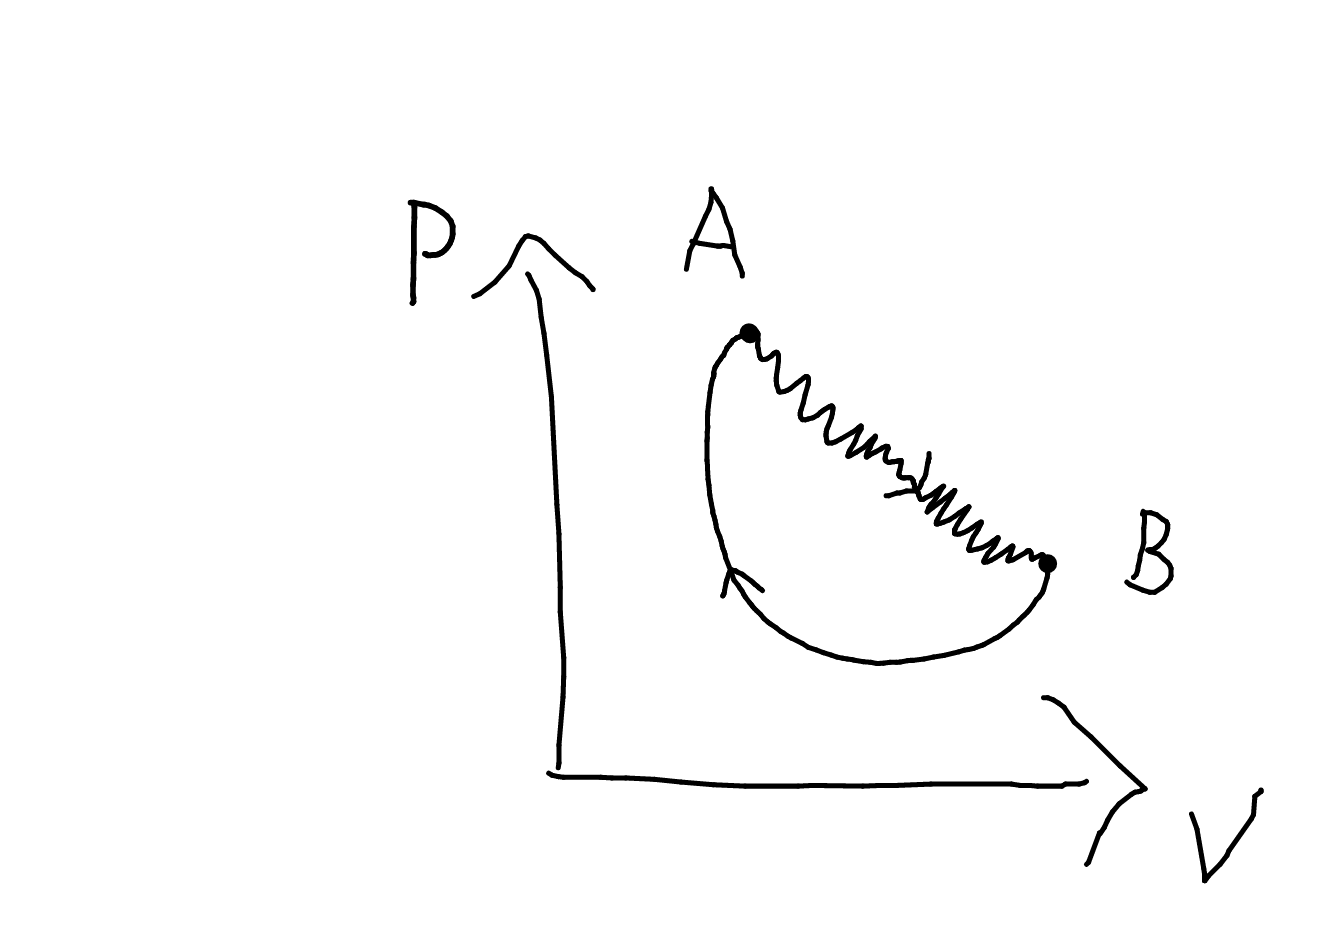
\includegraphics[width=0.5\textwidth]{TrasfAperta.png}
    \label{TrasformazioneAperta}
\end{figure}
Possiamo quindi applicare la disuguaglianza integrale nel caso generale esplicitando l'integrale:
\begin{equation}
\begin{split}
    \oint\frac{\delta Q}{T}&=\int_A^B\frac{\delta Q_{irr}}{T_S}+\int_B^A\frac{\delta Q_{rev}}{T}=\\
    &=\int_A^B\frac{\delta Q_{irr}}{T_S}+\int_B^A\dif S=\int_A^B\frac{\delta Q_{irr}}{T_S}-\int_A^B\dif S=\\
    &=\int_A^B\frac{\delta Q_{irr}}{T_S}-\left[S(B)-S(A)\right]\leq 0
\end{split}
\end{equation}
Otteniamo quindi:
\[\boxed{\int_A^B\frac{\delta Q_{irr}}{T_S}\leq S(B)-S(A)}\]
Che rappresenta la forma più generale della disuguaglianza di Clausius e rappresenta una formulazione matematica del secondo principio della termodinamica, includendo un importante risultato matematico (l'esistenza della funzione di stato \textbf{entropia}) e uno fisico (la disuguaglianza, ottenuta dall'enunciato di Kelvin).
\note Nel caso di n sorgenti vale invece:
\[\sum_i\frac{Q_i}{T_i}\leq S(B)-S(A)\]
Inoltre, essendo l'entropia una funzione di stato, è possibile calcolarla direttamente solo per trasformazioni reversibili, mentre per quelle \textbf{irreversibili} si può calcolare \textit{combinando le variazioni di entropia di altre due trasformazioni reversibili}.
\subsection{La Variazione di Entropia di Alcune Trasformazioni}
\paragraph{Solidi e Liquidi}
Durante le trasformazioni di fase il calore scambiato con una certa massa di sostanza vale:
\[Q=\pm m\lambda\]
Calcoliamo l'integrale di Clausius:
\begin{equation}
    \Delta S=\int \frac{\dif Q_{rev}}{T_0}=\frac{Q}{T_0}=\pm\frac{m\lambda}{T_0}
\end{equation}
Quando invece i solidi e liquidi passano da una temperatura all'altra:
\[\Delta S=\int_A^B\frac{\delta Q}{T}=mc\int_A^B\frac{\dif T}{T}=mc\ln\frac{T_B}{T_A}\]
\paragraph{Trasformazioni Reversibili dei Gas}
Per ogni trasformazioni reversibile possiamo applicare il seguente ragionamento:
\begin{equation}
\begin{split}
    \dif S&=\frac{\delta Q_{rev}}{T}=n\overline{c}_V\frac{\dif T}{T}+\frac{1}{T}p\dif V=\\
    &=n\overline{c}_V\frac{\dif T}{T}+\frac{1}{T}\frac{nRT}{V}\dif V=\\
    &=n\overline{c}_V\frac{\dif T}{T}+\frac{nR}{V}\dif V=n\overline{c}_V\frac{\dif T}{T}+nR\frac{\dif V}{V}=\\
    &=n\overline{c}_V\left[\frac{\dif T}{T}+\frac{\overline{c}_p-\overline{c}_V}{\overline{c}_V}\frac{\dif V}{V}\right]=\\
    &=n\overline{c}_V\left[\frac{\dif T}{T}+(\gamma-1)\frac{\dif V}{V}\right]
\end{split}
\end{equation}
Calcoliamo ora l'integrale di Clausius:
\begin{equation}
\begin{split}
    \Delta S&=\int_A^B\dif S=\int_A^Bn\overline{c}_V\left[\frac{\dif T}{T}+(\gamma-1)\frac{\dif V}{V}\right]=\\
    &=n\overline{c}_V\int_A^B\left[\frac{\dif T}{T}+(\gamma-1)\frac{\dif V}{V}\right]=\\
    &=n\overline{c}_V\left[\ln\frac{T_B}{T_A}+(\gamma-1)\ln\frac{V_B}{B_A}\right]=\\
    &=n\overline{c}_V\left[\ln\frac{T_B}{T_A}+\left(\ln\frac{V_B}{B_A}\right)^{\gamma-1}\right]=\\
    &=n\overline{c}_V\ln\left[\frac{T_B}{T_A}\left(\frac{V_B}{B_A}\right)^{\gamma-1}\right]=\\
    &=n\overline{c}_V\ln\left[\frac{T_BV_B^{\gamma-1}}{T_AV_A^{\gamma-1}}\right]
\end{split}
\end{equation}
Possiamo quindi esprimere in tre modi la variazione di entropia:
\[\Delta S=n\overline{c}_V\ln\left[\frac{T_BV_B^{\gamma-1}}{T_AV_A^{\gamma-1}}\right]=n\overline{c}_V\ln\left[\frac{p_BV_B^{\gamma}}{p_AV_A^{\gamma}}\right]=n\overline{c}_V\ln\left[\frac{T_A^{\gamma}T_B^{\gamma}}{p_A^{\gamma-1}p_B^{\gamma-1}}\right]\]
Esaminiamo ora singolarmente le maggiori trasformazioni reversibili.\\
L'\textbf{adiabatica} è la più semplice, in quanto è caratterizzata da $pV^{\gamma}=cost$, quindi otteniamo:
\[\Delta S=n\overline{c}_V\ln\left[\frac{p_BV_B^{\gamma}}{p_AV_A^{\gamma}}\right]=n\overline{c}_V\ln(1)=0\]
Ossia una trasformazione adiabatica è \textbf{isoentropica}, non cambia mai il proprio valore di Entropia.
Per quanto riguarda l'\textbf{isocora}:
\[\Delta S=n\overline{c}_V\ln\left[\frac{T_BV_B^{\gamma-1}}{T_AV_A^{\gamma-1}}\right]=n\overline{c}_V\ln\frac{T_B}{T_A}=n\overline{c}_V\ln\frac{p_B}{p_A}\]
L'\textbf{isobara}:
\[\Delta S=n\overline{c}_V\ln\left[\frac{p_BV_B^{\gamma}}{p_AV_A^{\gamma}}\right]=n\overline{c}_V\gamma\ln\frac{V_B}{V_A}=n\overline{c}_V(\frac{\overline{c}_p}{\overline{c}_V})\ln\frac{V_B}{V_A}=n\overline{c}_p\ln\frac{V_B}{V_A}=n\overline{c}_p\ln\frac{T_B}{T_A}\]
E infine l'\textbf{isoterma}:
\[\Delta S=n\overline{c}_V\ln\left[\frac{T_BV_B^{\gamma-1}}{T_AV_A^{\gamma-1}}\right]=n\overline{c}_V(\gamma-1)\ln\frac{V_B}{V_A}=n\overline{c}_V(
\frac{\overline{c}_p-\overline{c}_V}{\overline{c}_V})\ln\frac{V_B}{V_A}=n(\overline{c}_p-\overline{c}_V)\ln\frac{V_B}{V_A}=nR\ln\frac{V_B}{V_A}=nR\ln\frac{p_A}{p_B}\]
\paragraph{Espansione Libera}
Studiamo ora il caso dell'Espansione Libera di un gas come nel Secondo Esperimento di Joule. Siccome l'entropia è una funzione di stato possiamo applicare il risultato ottenuto anche ad una trasformazione irreversibile (come è tal caso) e otteniamo:
\begin{equation}
\Delta S=n\overline{c}_V\ln\left[\frac{T_fV_f^{\gamma-1}}{T_iV_i^{\gamma-1}}\right]=n\overline{c}_V\ln\frac{V_f^{\gamma-1}}{V_i^{\gamma-1}}=nR\ln\frac{V_f}{V_i}=nR\ln\frac{V_B+V_A}{V_A}>0
\end{equation}
Notiamo che la variazione di entropia è positiva, come ci si aspettava. 
\paragraph{Equilibrio Termico di due Corpi}
Dati due corpi a temperatura $T_A$ e $T_B$ rispettivamente, il calore che si scambiano è:
\[\delta Q_A=m_Ac_A\dif T\quad\delta Q_B=m_Bc_B\dif T\]
Calcoliamo l'integrale di Clausius tra lo stato iniziale e quello di equilibrio:
\[\Delta S=\Delta S_A+\Delta S_B=m_Ac_A\ln\frac{T_e}{T_A}+m_Bc_B\ln\frac{T_e}{T_B}\]
Si può dimostrare che in generale questa quantità è positiva utilizzando le proprietà dei logaritmi, considerando il caso in cui i corpi abbiano uguale massa e stesso calore specifico:
\begin{equation}
\begin{split}
    \Delta S&=mc\ln\left[\frac{(T_A+T_B)^2}{T_AT_B}\right]=\\
    &=2mc\ln\left[\frac{T_A+T_B}{\sqrt{T_AT_B}}\right]>0
\end{split}
\end{equation}
L'argomento è maggiore di 1 in quanto si può dimostrare che la media aritmetica è maggiore della media geometrica degli stessi valori. 

\paragraph{Tabella delle Trasformazioni Reversibili}
\begin{center}
\scalebox{1.5}{
\begin{tabular}{|c|c|c|c|c|}
    \hline
    \textbf{Trasformazione} & \textbf{Q} & \textbf{L} & \textbf{$\Delta U$} & \textbf{$\Delta S$}  \\
    \hline
    Isobara & $n\overline{c}_p\Delta T$ & $p_A(V_B-V_A)$ & $n\c_V\Delta T$ & $n\c_p\ln\frac{T_B}{T_A}$ \\
    \hline
    Isocora & $n\c_V\Delta T$ & 0 & $n\c_V\Delta$ & $n\c_v\ln\frac{T_B}{T_A}$\\
    \hline
    Isoterma & $L$ & $nRT\ln\frac{V_B}{V_A}$ & 0 & $nR\ln\frac{V_B}{V_A}$\\
    \hline
    Abiabatica & 0 & $-n\c_V\Delta T$ & $n\c_V\Delta T$ & 0\\
    \hline
\end{tabular}}
\end{center}

\end{document}